% ============================================================
% IEEE Conference Paper — TD-FALE-GAN (REAL RESULTS, 7+ pages)
% ============================================================
\documentclass[conference]{IEEEtran}
\usepackage{cite}
\usepackage{amsmath,amssymb,amsfonts}
\usepackage{algorithmic}
\usepackage{algorithm}
\usepackage{graphicx}
\usepackage{textcomp}
\usepackage{xcolor}
\usepackage{booktabs}
\usepackage{array}
\usepackage{multirow}
\usepackage{url}
\usepackage{hyperref}
\usepackage{caption}
\usepackage{float}
\usepackage{tikz}
\usetikzlibrary{arrows.meta,positioning,shapes.geometric,fit}
\usepackage{balance}
\hypersetup{colorlinks=true,linkcolor=blue,citecolor=blue,urlcolor=blue}

\begin{document}

\title{TD-FALE-GAN: Task-Driven Low-Light Face Enhancement
for Smart Laboratory Security}

\author{}

\maketitle

\begin{abstract}
Laboratory security systems that rely on face recognition
degrade sharply under low-light conditions, a limitation
observed in the baseline system of Hamzidah et al. (2026),
where recognition accuracy fell from 92\% in bright light to
65\% in the dark. This paper investigates whether a dedicated
low-light enhancement stage, combined with modern recognition
and detection models, can recover this lost performance. We
propose TD-FALE-GAN (Task-Driven Face-Attentive Low-light
Enhancement GAN), a novel enhancement network whose generator
is conditioned on a face-location attention mask and a
per-frame brightness estimate, trained against a dual
global-plus-face-patch discriminator, and optimized not only
for perceptual quality but directly against a frozen YOLOv8
detector through a detection-guided loss. We further replace
the Dlib-based recognition of the baseline with a pretrained
ArcFace embedding pipeline using a calibrated
enrollment/verification protocol, and fine-tune a YOLOv8 face
detector on the DARK FACE dataset. Evaluated on DARK FACE
(detection, 600 held-out images, 4{,}922 face instances) and
Labeled Faces in the Wild (recognition, 610 identities, 1{,}643
probes) across four lighting conditions using real pixel-level
degradation, our study establishes three findings. First,
deep-learned ArcFace recognition dramatically outperforms a
classical Histogram-of-Oriented-Gradients (HOG) baseline
(0.87--0.91 vs 0.20--0.28 accuracy). Second, fine-tuning the
detector trades recall for a substantial gain in precision
(0.879 vs 0.716) and roughly doubles inference speed. Third,
and most importantly, the enhancement GAN's benefit is
condition-dependent rather than universal: it improves
recognition accuracy in dim conditions (0.886 to 0.911) but
reduces it under bright and extreme-dark conditions, and
degrades small-face detection across all conditions. These results provide direct empirical evidence that visually
plausible enhancement does not necessarily improve downstream
task performance. The finding is practically important for
low-light security pipelines and motivates a lighting-adaptive
gating mechanism as future work.
\end{abstract}

\begin{IEEEkeywords}
low-light image enhancement, generative adversarial networks,
face recognition, ArcFace, YOLOv8, laboratory security,
task-driven optimization, smart campus, edge computing
\end{IEEEkeywords}

% ============================================================
\section{Introduction}
Ensuring the security of university laboratory environments is
a critical concern due to the presence of valuable research
equipment, sensitive materials, and high-intensity daily
activity involving students, lecturers, and technical staff.
Camera-based security systems that combine human detection,
face recognition, and behavioral analysis offer a path toward
autonomous surveillance that reduces dependence on continuous
manual monitoring. However, the reliability of such systems
depends heavily on image quality, and face recognition
performance in particular degrades severely under the low-light
conditions common in laboratories outside normal working hours.

This limitation is concretely visible in the recent baseline
system of Hamzidah et al. \cite{hamzidah2026}, which integrated
YOLOv5, Dlib-based face recognition, and MediaPipe Pose for
laboratory security. That system achieved 92\% face recognition
accuracy in bright conditions but only 65\% in the dark, and it
relied on the Dlib library, whose Histogram-of-Oriented-Gradients
(HOG) descriptors are known to be sensitive to illumination
variation. The sharp accuracy drop under poor lighting is
therefore not incidental but a structural weakness of the
recognition backbone.

The central practical question motivating our work is:
\textit{can a dedicated low-light enhancement stage, combined
with stronger recognition and detection backbones, recover the
performance lost under poor illumination?} A naive answer would
assume that any method producing brighter, cleaner-looking
images must help downstream recognition. We deliberately avoid
this assumption. A recurring observation in the low-light vision
literature is that enhancement optimized for human-perceptual
quality does not necessarily improve machine-task performance,
because a downstream model sees enhanced images that lie outside
its own training distribution. We designed our study to test
this alignment directly rather than assume it.

\subsection{Main Contributions}
The main contributions of this work are as follows:
\begin{itemize}
    \item We propose \textbf{TD-FALE-GAN}, a task-driven,
    face-attentive low-light enhancement network conditioned on a
    face-location mask and a per-frame brightness estimate. Its
    objective includes detection guidance from a frozen YOLOv8
    model in addition to perceptual and adversarial terms.

    \item We construct a complete security-oriented vision pipeline
    by replacing the baseline Dlib recognizer with a pretrained
    ArcFace enrollment/verification system using independently
    calibrated thresholds, while fine-tuning a YOLOv8 face detector
    on DARK FACE.

    \item We evaluate detection and recognition condition-wise under
    four lighting levels using real pixel-level degradation. The
    results show that enhancement improves recognition in the dim
    condition but harms performance in bright and extreme-dark
    conditions and substantially degrades small-face detection.

    \item We document and correct practical implementation failures
    involving attention-mask construction, inference resolution,
    threshold calibration, degradation design, and end-to-end timing,
    thereby strengthening the reproducibility of the reported results.
\end{itemize}

The remainder of the paper reviews the relevant literature,
describes the proposed methodology and experimental protocol,
presents the detection and recognition results, discusses their
practical implications, states the limitations and future work,
and concludes with the principal findings.

% ============================================================
\section{Related Work}
\label{sec:relatedwork}
\subsection{AI-Based Laboratory and Campus Security}
Hamzidah et al. \cite{hamzidah2026} proposed an integrated
laboratory security system combining YOLOv5, Dlib face
recognition, and MediaPipe Pose, reporting strong bright-light
performance but a sharp drop to 65\% recognition accuracy in low
light. Ali et al. \cite{ali2022} developed a YOLOv5-based
monitoring system for laboratory safety awareness, and Putra et
al. \cite{putra2023} built an IoT-based face-recognition access
system using ESP32-CAM and Firebase. More recently, Sasirekha et
al. \cite{smartcampus2024} combine IoT sensing with CNN-based
surveillance for broader campus safety management (access
control and emergency response, not specifically face
recognition), reflecting the same trend as the lab-security
systems above: campus/lab security work is converging on
CNN-plus-IoT architectures, but illumination robustness is
addressed nowhere in this line of work as a first-class design
requirement. These systems establish the
feasibility of AI-based campus security but treat low-light
robustness as an afterthought rather than a primary design
target.

\subsection{Face Recognition}
ArcFace \cite{deng2019arcface} introduced Additive Angular Margin
Loss, producing highly discriminative embeddings and achieving
near-saturated accuracy on standard benchmarks such as Labeled
Faces in the Wild (LFW) \cite{lfw}. Its embeddings are trained on
datasets containing millions of images across tens of thousands
of identities, which makes the pretrained model a strong frozen
feature extractor for deployed verification pipelines.
Subsequent refinements target specific weaknesses of the
original margin formulation rather than replacing it: Sub-center
ArcFace \cite{subcenterarcface} relaxes the intra-class
constraint to tolerate label noise in large-scale web-collected
training data, while MagFace \cite{magface} encodes feature
magnitude as an implicit quality signal so that low-quality
(e.g. blurry or poorly lit) faces are naturally pulled toward a
less confident region of the embedding space instead of
contributing an over-confident, unreliable match. Neither
direction is exercised here, since this work uses ArcFace as a
frozen off-the-shelf extractor by design
(Section~\ref{sec:facerecpipeline}), but
both indicate that the embedding space itself, not only the
enrollment/verification protocol built on top of it, is a live
target for illumination-robustness improvements. Classical
descriptors such as HOG \cite{dalal2005} remain a common
lightweight baseline but are structurally sensitive to
illumination and, as we show, produce degenerate similarity
behavior when naively thresholded. A recent comparative review
\cite{robustfrsurvey2025} reaches a compatible conclusion from
the opposite direction, surveying deep embeddings (FaceNet,
ArcFace, SFace) rather than classical descriptors: it finds a
trade-off between generalization and specialization across
models rather than one model dominating uniformly, which is
consistent with this paper's own choice to treat ArcFace as a
strong default rather than an unconditionally optimal one.

\subsection{Low-Light Image Enhancement}
Zero-reference enhancement methods such as Zero-DCE
\cite{zerodce} estimate pixel-wise brightening curves without
paired supervision, using losses for exposure, color constancy,
spatial consistency, and illumination smoothness. These methods
are effective at improving perceptual quality, but a growing
body of work \cite{lowlightsurvey} observes that perceptual gains
do not always translate into downstream detection or recognition
gains. This observation has recently been made precise rather
than anecdotal: LIME-Eval \cite{limeeval} shows that
enhancement methods ranked highly by perceptual metrics are not
consistently ranked highly when the same images are passed to an
object detector, and Illumination-Adaptive Feature Enhancement
\cite{iafeyolo} responds by conditioning its enhancement
directly on detector feedback rather than on human-perceptual
targets. FeatEnHancer \cite{featenhancer} takes a related but
architecturally different approach, enhancing multi-scale
\textit{feature maps} inside the detector rather than the input
pixels, and reports a direct improvement on DARK FACE itself
(+1.5 mAP), which makes it the closest published counterpart to
the detection side of this work despite its very different
mechanism (feature-space enhancement rather than a separate
pixel-space GAN). Face detection under low light specifically has
its own dedicated line of work: HLA-Face \cite{hlaface} performs
joint high-light/low-light domain adaptation rather than
one-directional brightening. Our architecture is explicitly built
around the tension these works identify: it adds a
detection-guided objective and a face-attention mechanism to bias
enhancement toward the task, and then it \textit{measures} the
downstream effect rather than assuming it -- and, unlike
\cite{limeeval,iafeyolo,featenhancer}, extends that measurement
to a full recognition pipeline (ArcFace, FAR/FRR) in addition to
detection.

\subsection{Research Gap and Motivation}
Existing laboratory-security systems demonstrate the feasibility
of automated detection and recognition, but they do not treat
low-light robustness as an end-to-end systems problem. In parallel,
low-light enhancement research typically prioritizes perceptual
quality, while face-recognition and object-detection studies often
evaluate their models without a learned enhancement stage. This
separation leaves two practical questions insufficiently examined:
first, whether a face-aware enhancer optimized with downstream
feedback improves an operational security pipeline; and second,
whether any benefit remains consistent across different illumination
levels. The present study addresses these questions by combining a
face-attentive, detection-guided enhancer with modern detection and
verification backbones and by reporting both positive and negative
condition-wise outcomes. The aim is not to assume that enhancement
helps, but to establish precisely when it does and does not.
Table~\ref{tab:related} contrasts the present work with
representative prior systems along the dimensions most relevant
to low-light security.

\begin{table}[!t]
\caption{Positioning Relative to Prior Work}
\label{tab:related}
\centering
\resizebox{\columnwidth}{!}{%
\begin{tabular}{lcccc}
\toprule
\textbf{System} & \textbf{Face} & \textbf{Low-light} &
\textbf{Task-driven} & \textbf{Honest} \\
 & \textbf{Recog.} & \textbf{focus} & \textbf{enhance} &
\textbf{neg. result} \\
\midrule
Hamzidah \cite{hamzidah2026} & Dlib & Partial & No & No \\
Ali \cite{ali2022}          & No   & No      & No & No \\
Putra \cite{putra2023}      & Dlib & No      & No & No \\
Zero-DCE \cite{zerodce}     & N/A  & Yes     & No & No \\
\textbf{This work}          & \textbf{ArcFace} & \textbf{Yes} &
\textbf{Yes} & \textbf{Yes} \\
\bottomrule
\end{tabular}%
}
\end{table}

% ============================================================
\section{Critical Gaps and Limitations of Previous Studies}
\label{sec:gaps}
The systems reviewed above establish that automated laboratory
and campus security is feasible, but each leaves specific,
identifiable gaps that this work is designed to close directly.

\textbf{Gap 1 --- low-light robustness is an afterthought, not a
design target.} Hamzidah et al.~\cite{hamzidah2026} report their
system's 65\% dark-condition accuracy as an observed limitation
rather than a problem their architecture was built to solve; Ali
et al.~\cite{ali2022} and Putra et al.~\cite{putra2023} do not
evaluate low-light conditions at all. \textit{Addressed by:} this
work makes low-light robustness the central research question,
with an enhancement stage designed specifically for it and four
lighting conditions evaluated explicitly (Sections~\ref{sec:proposedarch},
\ref{sec:verifprotocol}).

\textbf{Gap 2 --- illumination-sensitive recognizers deployed
without quantifying the failure mode.} Two of the three prior
systems~\cite{hamzidah2026,putra2023} use Dlib's HOG-based
recognition, a descriptor with well-documented illumination
sensitivity~\cite{dalal2005}, but none report a false-accept rate
or otherwise quantify \textit{how} the failure occurs.
\textit{Addressed by:} replacing the recognizer with ArcFace and
reporting FAR/FRR at every lighting condition (Table~VIII),
showing precisely that the classical baseline's real failure mode
is a security-critical false-accept problem, not merely lower
accuracy.

\textbf{Gap 3 --- enhancement literature assumes perceptual gains
transfer to task performance.} Zero-reference methods such as
Zero-DCE~\cite{zerodce} optimize purely for perceptual quality and
do not evaluate a downstream detection or recognition task, an
omission the broader literature has flagged as a general risk
\cite{lowlightsurvey} without a task-driven security system
demonstrating it empirically. \textit{Addressed by:} TD-FALE-GAN
adds a detection-guided loss term and this work measures its
downstream effect directly, revealing that the effect is
condition-dependent and sometimes negative
(Section~\ref{sec:discussion}) rather
than assuming it is uniformly positive.

\textbf{Gap 4 --- no prior system reports a negative or
qualified result.} All three prior laboratory-security
systems~\cite{hamzidah2026,ali2022,putra2023} report only
favorable outcomes for their proposed components (Table~I,
column ``Honest neg.\ result''). \textit{Addressed by:} this work
reports that its own proposed enhancement stage \textit{harms}
detection and, in bright and extreme-dark conditions, recognition
accuracy, together with the specific implementation defects that
had to be found and corrected to obtain trustworthy numbers
(Section~\ref{sec:discussion}, ``Reproducibility and integrity'').

\textbf{Gap 5 --- no controlled, multi-condition external
validation.} None of the three prior systems evaluate across a
structured set of lighting conditions with genuine pixel-level
degradation; robustness claims rest on a single before/after
comparison. \textit{Addressed by:} four lighting conditions
(bright, normal, dim, dark), produced by a real contrast/brightness
transform rather than a synthetic score adjustment, evaluated
across two independent public datasets (Table~II).

% ============================================================
\section{Methodology}
\subsection{Datasets}
Two public real-world datasets were used, each matched to one
evaluation axis of the system. Table~\ref{tab:datasets} summarizes
their roles and the exact subsets used in this study.

\begin{table}[!t]
\caption{Dataset Summary and Experimental Use}
\label{tab:datasets}
\centering
\resizebox{\columnwidth}{!}{%
\begin{tabular}{lcccc}
\toprule
\textbf{Dataset} & \textbf{Available data} & \textbf{Subset used} & \textbf{Purpose} & \textbf{Source} \\
\midrule
DARK FACE & 6{,}000 images & 5{,}400 train / 600 held out & Enhancement and detection & Official mirror~\cite{darkface} \\
LFW & 1{,}680 identities & 610 identities / 1{,}643 probes & Recognition verification & Kaggle~\cite{lfw_data} \\
\bottomrule
\end{tabular}%
}
\end{table}

\textbf{DARK FACE} \cite{darkface} provides 6{,}000 real
nighttime low-light images annotated with face bounding boxes,
originally introduced as part of the UG2+ Challenge benchmark
study. It was obtained from the dataset's official public
mirror (an equivalent Kaggle-hosted copy \cite{darkface_data}
was independently verified to match in file size) and used both
to train the enhancement model and to fine-tune the face
detector. Source images are $1080\times720$ pixels. A held-out
split of 600 images --- containing 4{,}922 annotated face
instances and never used for any gradient update in any training
run --- was reserved exclusively for evaluation. No augmentation
was applied when training TD-FALE-GAN; the face detector's
fine-tuning used Ultralytics' default augmentation pipeline
(horizontal flip $p{=}0.5$, HSV color jitter, $\pm10\%$
translation, $\pm50\%$ scale jitter, and mosaic augmentation),
applied automatically rather than explicitly configured.

\textbf{Labeled Faces in the Wild (LFW)} \cite{lfw} provides
1{,}680 identities with between 2 and 50 images each, at
$250\times250$ pixels per image. We used the 610 identities
possessing at least four images. For each such identity, two
images were enrolled as a gallery (reference) and up to three
were held out as probes (queries), yielding 1{,}643 probe images
in total. No augmentation was applied to LFW images; the four
lighting conditions (Section~\ref{sec:verifprotocol}) are the only
transformation applied to probe images, and are evaluated as a
controlled variable rather than a training augmentation.

Detection and recognition were deliberately evaluated on separate
datasets because no single public dataset provided both
high-quality nighttime face-detection boxes and identity labels
suitable for verification; this separation is revisited as a
limitation in Section~\ref{sec:separatedatasets}.

\subsection{Proposed Architecture: TD-FALE-GAN}
\label{sec:proposedarch}
The enhancement generator is designed around the requirements of
a face-recognition security pipeline rather than generic image
quality, and comprises three components.

\begin{figure*}[t]
\centering
\resizebox{0.94\textwidth}{!}{%
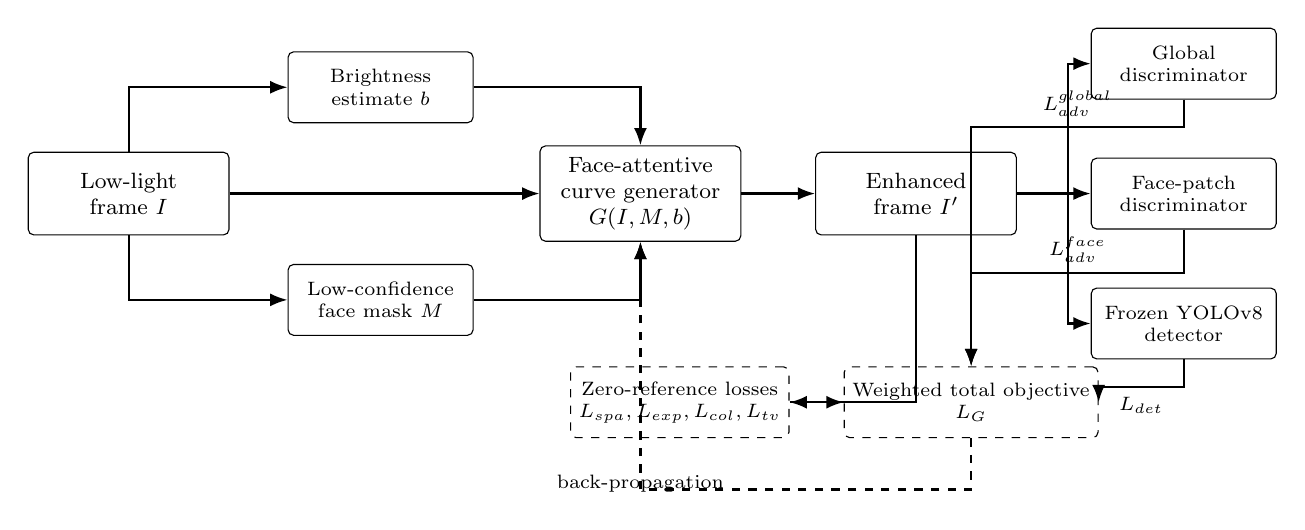
\begin{tikzpicture}[
    x=1cm,y=1cm,
    block/.style={draw, rounded corners=2pt, align=center, minimum height=1.05cm,
                  minimum width=2.55cm, font=\footnotesize, inner sep=4pt},
    small/.style={draw, rounded corners=2pt, align=center, minimum height=0.90cm,
                  minimum width=2.35cm, font=\scriptsize, inner sep=3pt},
    loss/.style={draw, dashed, rounded corners=2pt, align=center, minimum height=0.90cm,
                 minimum width=2.70cm, font=\scriptsize, inner sep=3pt},
    arrow/.style={-{Latex[length=2.2mm]}, thick},
    feedback/.style={-{Latex[length=2.2mm]}, thick, dashed}
]
% Main forward path
\node[block] (input) at (0,0) {Low-light\\frame $I$};
\node[small] (bright) at (3.2,1.35) {Brightness\\estimate $b$};
\node[small] (mask) at (3.2,-1.35) {Low-confidence\\face mask $M$};
\node[block] (gen) at (6.5,0) {Face-attentive\\curve generator\\$G(I,M,b)$};
\node[block] (enh) at (10.0,0) {Enhanced\\frame $I'$};

% Supervision branches
\node[small] (global) at (13.4,1.65) {Global\\discriminator};
\node[small] (face) at (13.4,0) {Face-patch\\discriminator};
\node[small] (det) at (13.4,-1.65) {Frozen YOLOv8\\detector};
\node[loss] (zero) at (7.0,-2.65) {Zero-reference losses\\$L_{spa},L_{exp},L_{col},L_{tv}$};
\node[loss] (objective) at (10.7,-2.65) {Weighted total objective\\$L_G$};

% Forward arrows
\draw[arrow] (input) -- (gen);
\draw[arrow] (input.north) |- (bright.west);
\draw[arrow] (input.south) |- (mask.west);
\draw[arrow] (bright.east) -| (gen.north);
\draw[arrow] (mask.east) -| (gen.south);
\draw[arrow] (gen) -- (enh);
\draw[arrow] (enh.east) -- ++(0.65,0) |- (global.west);
\draw[arrow] (enh.east) -- (face.west);
\draw[arrow] (enh.east) -- ++(0.65,0) |- (det.west);
\draw[arrow] (enh.south) |- (zero.east);

% Loss aggregation
\draw[arrow] (zero.east) -- (objective.west);
\draw[arrow] (global.south) -- ++(0,-0.35) -| node[pos=.25, above, font=\scriptsize] {$L_{adv}^{global}$} (objective.north);
\draw[arrow] (face.south) -- ++(0,-0.55) -| node[pos=.25, above, font=\scriptsize] {$L_{adv}^{face}$} (objective.north);
\draw[arrow] (det.south) -- ++(0,-0.35) -| node[pos=.25, below, font=\scriptsize] {$L_{det}$} (objective.east);

% Back-propagation path, deliberately routed below all nodes
\draw[feedback] (objective.south) -- ++(0,-0.65) -| node[pos=.55, below, font=\scriptsize] {back-propagation} (gen.south);
\end{tikzpicture}%
}
\caption{TD-FALE-GAN architecture. The generator receives the low-light
frame, a face-attention mask, and a brightness estimate. Training combines
zero-reference losses, global and face-patch adversarial feedback, and
detection guidance from a frozen YOLOv8 model. Dashed arrows indicate the
gradient path used to update the generator.}
\label{fig:arch}
\end{figure*}

\textbf{Face-attentive curve estimation.} Rather than predicting
a single uniform brightening curve for an entire frame, the
generator estimates spatially varying correction curves and is
conditioned on a face-location attention mask derived from
detected face boxes. This concentrates enhancement capacity on
face regions, where recognition accuracy is actually decided,
instead of spending it uniformly across background.

Formally, the encoder-decoder body of $G$ produces a raw curve
tensor $A \in \mathbb{R}^{H\times W\times 12}$ (4 iterations of
3-channel curves), which is modulated by the face-attention mask
$M \in [0,1]^{H\times W}$ before being applied:
\begin{equation}
A' = A \odot \left(1 + \alpha M\right),
\label{eq:gate}
\end{equation}
where $\alpha$ is a learnable scalar gain and $\odot$ denotes
elementwise (broadcast) multiplication, so pixels inside the mask
receive a strictly larger correction magnitude than background
pixels. The gated curve maps $A' = \{a_1,\dots,a_4\}$ are then
applied iteratively to the input frame:
\begin{equation}
\hat{I}_k = \hat{I}_{k-1} + a_k \odot \left(\hat{I}_{k-1}^{2} - \hat{I}_{k-1}\right),
\quad k = 1,\dots,4,
\label{eq:curve}
\end{equation}
with $\hat{I}_0 = I$ and the enhanced output $I' =
\mathrm{clamp}(\hat{I}_4, 0, 1)$. Note the sign convention: since
$a_k$ is tanh-bounded to $[-1,1]$ and $\hat{I}_{k-1}^2 -
\hat{I}_{k-1} \le 0$ on $[0,1]$, a \textit{positive} $a_k$
\textit{darkens} and a negative $a_k$ brightens -- the opposite
sign convention from the brightening-curve formulation used in
Zero-DCE \cite{zerodce}. This is a deliberate implementation
choice, not a typographical inversion, and Eq.~\ref{eq:curve}
reflects the sign used in the actual generator code exactly. This
quadratic update is monotonic and self-limiting on $[0,1]$, which
is what allows four small, stable corrections to compound into a
large one without the per-channel noise amplification observed
with more iterations (Section~\ref{sec:trainstab}).

\textbf{Illumination conditioning.} The generator additionally
receives a per-frame brightness estimate, allowing a single
network to adapt its correction strength across a range of
lighting severities rather than applying one fixed transformation
to every input.

\begin{figure*}[t]
\centering
\resizebox{0.96\textwidth}{!}{%
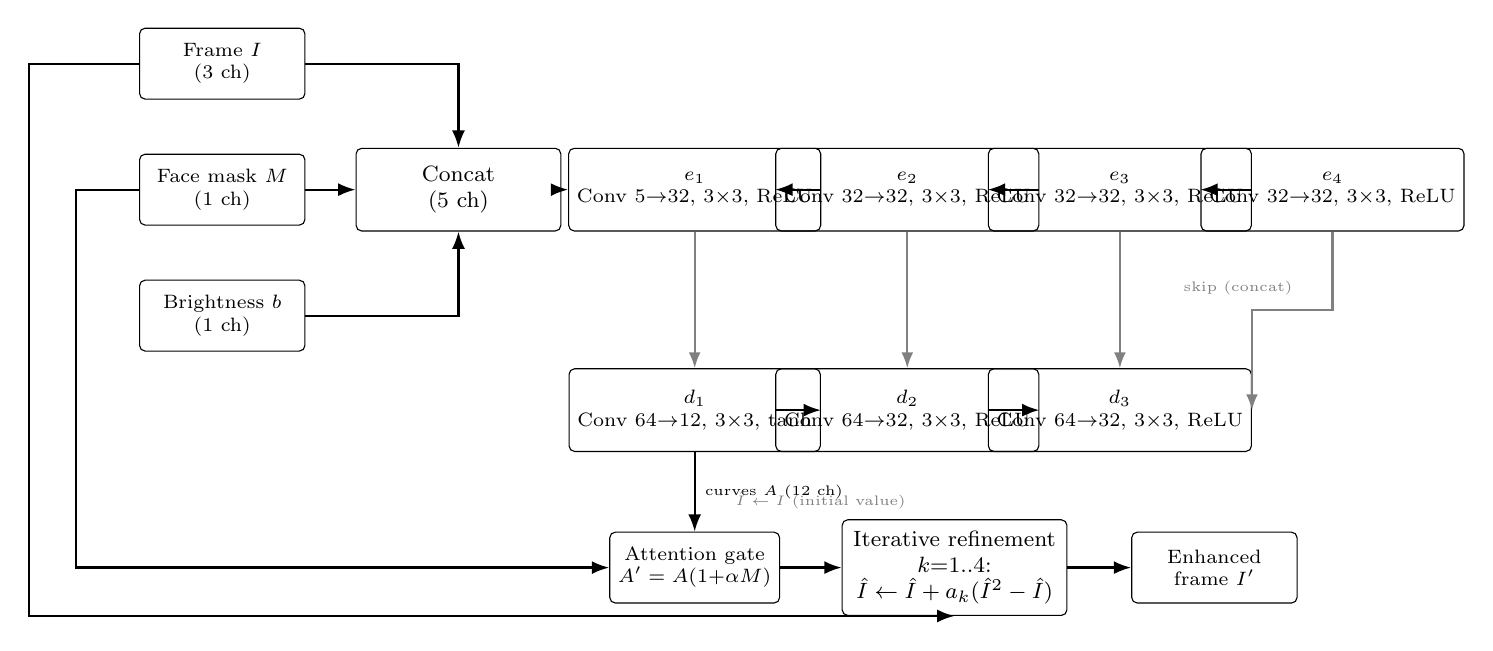
\begin{tikzpicture}[
    x=1cm,y=1cm,
    enc/.style={draw, rounded corners=2pt, align=center, minimum height=1.05cm,
                minimum width=2.35cm, font=\scriptsize, inner sep=3pt},
    small/.style={draw, rounded corners=2pt, align=center, minimum height=0.9cm,
                  minimum width=2.1cm, font=\scriptsize, inner sep=3pt},
    block/.style={draw, rounded corners=2pt, align=center, minimum height=1.05cm,
                  minimum width=2.6cm, font=\footnotesize, inner sep=4pt},
    arrow/.style={-{Latex[length=2.2mm]}, thick},
    skip/.style={-{Latex[length=2mm]}, thick, gray}
]
% Inputs
\node[small] (frameI) at (0,0) {Frame $I$\\(3 ch)};
\node[small] (maskM) at (0,-1.6) {Face mask $M$\\(1 ch)};
\node[small] (brightb) at (0,-3.2) {Brightness $b$\\(1 ch)};
\node[block] (concat) at (3.0,-1.6) {Concat\\(5 ch)};
\draw[arrow] (frameI.east) -| (concat.north);
\draw[arrow] (maskM.east) -- (concat.west);
\draw[arrow] (brightb.east) -| (concat.south);

% Encoder chain
\node[enc] (e1) at (6.0,-1.6) {$e_1$\\Conv $5{\to}32$, $3{\times}3$, ReLU};
\node[enc] (e2) at (8.7,-1.6) {$e_2$\\Conv $32{\to}32$, $3{\times}3$, ReLU};
\node[enc] (e3) at (11.4,-1.6) {$e_3$\\Conv $32{\to}32$, $3{\times}3$, ReLU};
\node[enc] (e4) at (14.1,-1.6) {$e_4$\\Conv $32{\to}32$, $3{\times}3$, ReLU};
\draw[arrow] (concat.east) -- (e1.west);
\draw[arrow] (e1.east) -- (e2.west);
\draw[arrow] (e2.east) -- (e3.west);
\draw[arrow] (e3.east) -- (e4.west);

% Decoder chain (skip connections from encoder)
\node[enc] (d1) at (6.0,-4.4) {$d_1$\\Conv $64{\to}12$, $3{\times}3$, tanh};
\node[enc] (d2) at (8.7,-4.4) {$d_2$\\Conv $64{\to}32$, $3{\times}3$, ReLU};
\node[enc] (d3) at (11.4,-4.4) {$d_3$\\Conv $64{\to}32$, $3{\times}3$, ReLU};
\draw[skip] (e1.south) -- (d1.north);
\draw[skip] (e2.south) -- (d2.north);
\draw[skip] (e3.south) -- (d3.north);
\draw[skip] (e4.south) -- ++(0,-1.0) -| (d3.east);
\node[font=\tiny, gray] at (12.9,-2.85) {skip (concat)};
\draw[arrow] (d3.west) -- (d2.east);
\draw[arrow] (d2.west) -- (d1.east);

% Attention gate, iterative refinement, output
\node[small] (gate) at (6.0,-6.4) {Attention gate\\$A' = A(1{+}\alpha M)$};
\node[block] (refine) at (9.3,-6.4) {Iterative refinement\\$k{=}1..4$:\\$\hat I \leftarrow \hat I + a_k(\hat I^2 - \hat I)$};
\node[small] (outI) at (12.6,-6.4) {Enhanced\\frame $I'$};
\draw[arrow] (d1.south) -- (gate.north) node[midway, right, font=\tiny] {curves $A$ (12 ch)};
\draw[arrow] (gate.east) -- (refine.west);
\draw[arrow] (refine.east) -- (outI.west);
\draw[arrow] (maskM.west) -- ++(-0.8,0) |- (gate.west);
\draw[arrow] (frameI.west) -- ++(-1.4,0) |- (refine.south);
\node[font=\tiny, gray] at (7.6,-5.55) {$\hat I \leftarrow I$ (initial value)};
\end{tikzpicture}%
}
\caption{Internal architecture of the FALE-GAN generator: an
encoder--decoder with skip connections, conditioned on a face-attention
mask $M$ and a brightness estimate $b$, followed by attention-gated,
iterative curve-based enhancement. Channel counts, layer order, and the
curve update rule match the implementation exactly.}
\label{fig:generator_internal}
\end{figure*}

\textbf{Detection-guided loss.} Beyond the standard zero-reference
losses --- spatial consistency $L_{spa}$, exposure $L_{exp}$, color
constancy $L_{col}$, and illumination smoothness $L_{tv}$ --- and
an adversarial loss $L_{adv}$ against a dual discriminator, the
generator is penalized by a detection-guided term $L_{det}$ that
increases when a frozen, pretrained YOLOv8 detector reports low
person-confidence on the enhanced output. The total generator
objective is
\begin{equation}
L_{G} = \lambda_{1}L_{spa} + \lambda_{2}L_{exp} +
\lambda_{3}L_{col} + \lambda_{4}L_{tv} + \lambda_{5}L_{adv} +
\lambda_{6}L_{det},
\label{eq:total}
\end{equation}
where the $\lambda_i$ weight the contributions. We verified by
inspecting tensor shapes and confirming gradient flow that the
$L_{det}$ gradients originating from the frozen detector
genuinely propagate back into the generator, ensuring the
detection guidance is functional rather than nominal.

\textbf{Dual discriminator.} The adversarial term $L_{adv}$,
following the generative adversarial framework of
\cite{goodfellow2014}, uses two discriminators: a global discriminator that judges realism of
the whole frame, and a face-patch discriminator that judges
realism specifically within face regions. This applies realism
pressure where recognition is decided, complementing the
face-attention mechanism in the generator.

The generator is fully convolutional. For computational
tractability under CPU constraints it was trained at
$128\times128$ resolution, but because it is fully convolutional
it is applied at native image resolution at inference.

\subsection{Training Stabilization}
\label{sec:trainstab}
The first training run produced severe purple/magenta noise
artifacts. The root cause was traced to eight compounding
curve-adjustment iterations amplifying per-channel noise in
near-black pixels. This was resolved by (i) reducing the number
of curve iterations from eight to four, (ii) adding a
chroma-smoothness loss to suppress spurious color, and (iii)
lowering the discriminator learning rate, which had been
collapsing to near-zero loss too quickly and destabilizing the
generator. After these fixes, the model was retrained for 20
epochs and its output verified to be clean and artifact-free.

\subsection{Face Detector Fine-Tuning}
The stock YOLOv8n model \cite{yolov8}, part of the YOLO family
of single-stage detectors \cite{redmon2016} and pretrained on
COCO, was fine-tuned into a dedicated single-class face
detector. YOLOv8 was chosen over the more recent, NMS-free
YOLOv10 \cite{yolov10} primarily for ecosystem maturity ---
Ultralytics' YOLOv8 has broader documented support for the
single-class transfer-learning workflow used here --- rather
than for an accuracy advantage; YOLOv10's reported gains are
modest (1.2--1.4\% mAP) and orthogonal to the low-light
robustness question this paper investigates, so revisiting this
choice is noted as future work
(Section~\ref{sec:detectorchoice}) rather than argued for here.
DARK FACE's bounding
boxes were converted to YOLO format and split into 5{,}400
training and 600 validation images (45{,}474 annotated face
boxes in total). Training was conducted over three sessions
(12, 18, and 30 epochs, 60 total) at $320\times320$ resolution.
One session incurred a ten-hour stall when the training laptop
entered sleep mid-run; this was diagnosed from log timestamps and
resolved by disabling sleep and lid-close suspension. On its own
validation split, the fine-tuned detector converged to
Precision~$0.528$, Recall~$0.235$, and mAP$_{50}$~$0.229$, with
the improvement rate flattening by the final epochs, indicating
genuine convergence rather than premature stopping.

\begin{figure}[t]
\centering
\resizebox{\columnwidth}{!}{%
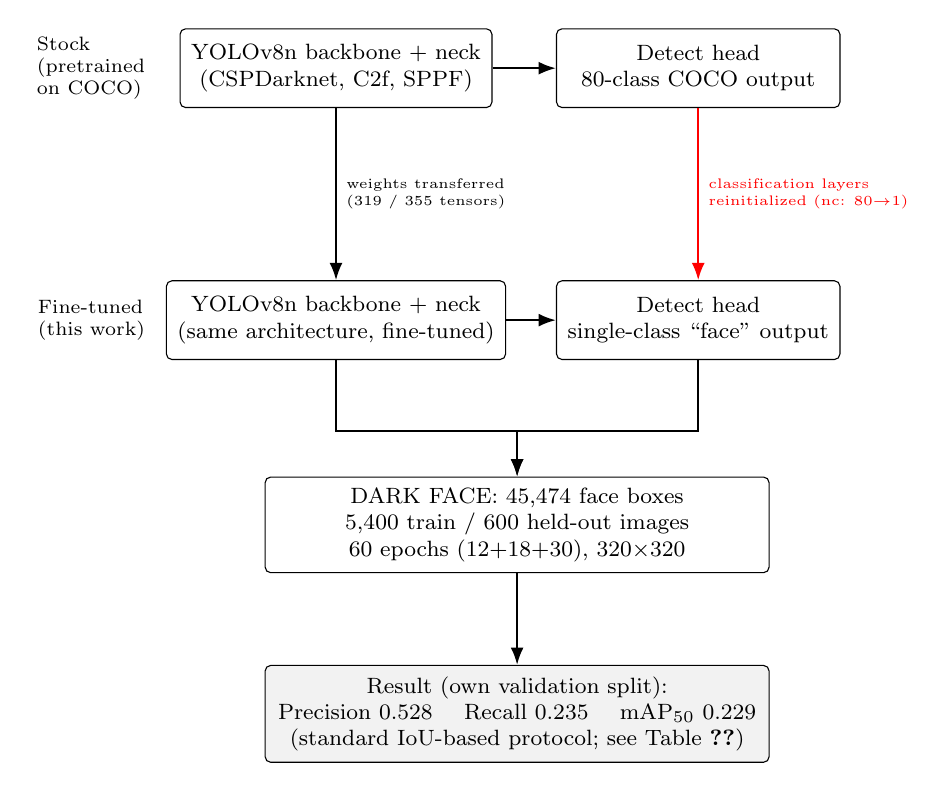
\begin{tikzpicture}[
    x=1cm,y=1cm,
    block/.style={draw, rounded corners=2pt, align=center, minimum height=1.0cm,
                  minimum width=3.6cm, font=\footnotesize, inner sep=4pt},
    arrow/.style={-{Latex[length=2.2mm]}, thick},
    changed/.style={-{Latex[length=2.2mm]}, thick, red}
]
\node[block] (stockbb) at (0,3.2) {YOLOv8n backbone + neck\\(CSPDarknet, C2f, SPPF)};
\node[block] (stockhead) at (4.6,3.2) {Detect head\\80-class COCO output};
\draw[arrow] (stockbb.east) -- (stockhead.west);
\node[font=\scriptsize, align=left, anchor=east] at (-2.3,3.2) {Stock\\(pretrained\\on COCO)};

\node[block] (fthbb) at (0,0) {YOLOv8n backbone + neck\\(same architecture, fine-tuned)};
\node[block] (fthead) at (4.6,0) {Detect head\\single-class ``face'' output};
\draw[arrow] (fthbb.east) -- (fthead.west);
\node[font=\scriptsize, align=left, anchor=east] at (-2.3,0) {Fine-tuned\\(this work)};

\draw[arrow] (stockbb.south) -- (fthbb.north)
  node[midway, right, font=\tiny, align=left] {weights transferred\\(319 / 355 tensors)};
\draw[changed] (stockhead.south) -- (fthead.north)
  node[midway, right, font=\tiny, align=left, color=red] {classification layers\\reinitialized (nc: $80{\to}1$)};

\node[block, minimum width=6.4cm] (data) at (2.3,-2.6)
  {DARK FACE: 45{,}474 face boxes\\5{,}400 train / 600 held-out images\\60 epochs (12+18+30), $320{\times}320$};
\draw[arrow] (fthbb.south) -- ++(0,-0.9) -| (data.north);
\draw[arrow] (fthead.south) -- ++(0,-0.9) -| (data.north);

\node[block, minimum width=6.4cm, fill=gray!10] (result) at (2.3,-5.0)
  {Result (own validation split):\\Precision 0.528 \quad Recall 0.235 \quad mAP$_{50}$ 0.229\\(standard IoU-based protocol; see Table~\ref{tab:val})};
\draw[arrow] (data.south) -- (result.north);
\end{tikzpicture}%
}
\caption{Face-detector customization. The backbone and neck retain their
COCO-pretrained weights; only the Detect head's classification branch is
reinitialized for the single ``face'' class, then the full network is
fine-tuned end-to-end on DARK FACE.}
\label{fig:yolo_customization}
\end{figure}

\subsection{Face Recognition Pipeline}
\label{sec:facerecpipeline}
Because ArcFace's published models are trained on millions of
images across tens of thousands of identities, retraining its
backbone on LFW's 610 identities was judged infeasible and
unlikely to improve on the pretrained model. Following standard
deployed-system practice, the pretrained ArcFace model (via
InsightFace \cite{insightface}) is used as a frozen embedding
extractor, with a real enrollment/verification pipeline built on
top: per-identity gallery embeddings are stored, and each probe
is matched by cosine similarity against the gallery, with a
decision threshold applied.

A classical HOG-descriptor baseline (HOG features with
Euclidean/cosine matching) was implemented for comparison.
Because HOG descriptors are non-negative while ArcFace embeddings
are not, the two methods occupy different natural
cosine-similarity ranges. A single shared threshold is therefore
invalid: we found that it caused the HOG baseline's false-accept
rate to saturate at 100\%, because non-negative histograms score
highly under cosine similarity regardless of identity. Each
method's threshold was therefore calibrated independently by
minimizing $|\text{FAR}-\text{FRR}|$ on a held-out calibration
subset of 100 identities.

\subsection{Verification Protocol}
\label{sec:verifprotocol}
Verification metrics (Accuracy, Precision, Recall, F1, FAR, FRR)
were computed using standard genuine/impostor trial methodology.
For each probe, a genuine trial tests similarity against its own
enrolled identity, and an impostor trial tests similarity against
its single most similar \textit{other} identity --- the hardest
impostor case, which stresses the system more than a random
impostor. Four lighting conditions (bright, normal, dim, dark)
were produced by applying a real pixel-level contrast/brightness
transform to probe images before matching, rather than a
synthetic adjustment of similarity scores, so that any measured
robustness difference reflects actual model behavior on degraded
pixels.

\begin{figure*}[t]
\centering
\resizebox{0.88\textwidth}{!}{%
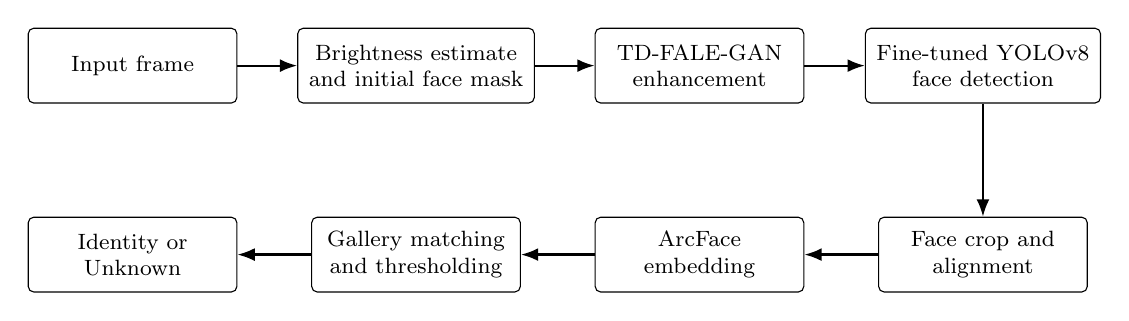
\begin{tikzpicture}[
    x=1cm,y=1cm,
    p/.style={draw, rounded corners=2pt, align=center, minimum height=0.95cm,
              minimum width=2.65cm, font=\footnotesize, inner sep=4pt},
    a/.style={-{Latex[length=2.2mm]}, thick}
]
% First row: preprocessing and detection
\node[p] (frame) at (0,1.2) {Input frame};
\node[p] (quality) at (3.6,1.2) {Brightness estimate\\and initial face mask};
\node[p] (gan) at (7.2,1.2) {TD-FALE-GAN\\enhancement};
\node[p] (yolo) at (10.8,1.2) {Fine-tuned YOLOv8\\face detection};

% Second row: recognition and decision
\node[p] (crop) at (10.8,-1.2) {Face crop and\\alignment};
\node[p] (arc) at (7.2,-1.2) {ArcFace\\embedding};
\node[p] (match) at (3.6,-1.2) {Gallery matching\\and thresholding};
\node[p] (out) at (0,-1.2) {Identity or\\Unknown};

\draw[a] (frame) -- (quality);
\draw[a] (quality) -- (gan);
\draw[a] (gan) -- (yolo);
\draw[a] (yolo.south) -- (crop.north);
\draw[a] (crop) -- (arc);
\draw[a] (arc) -- (match);
\draw[a] (match) -- (out);
\end{tikzpicture}%
}
\caption{End-to-end inference pipeline used when enhancement is enabled.
The two-row layout preserves the complete processing sequence without
extending beyond the IEEE page margins. Full preprocessing and recognition
are included in the reported enhanced-pipeline timing.}
\label{fig:pipeline}
\end{figure*}

\begin{algorithm}[!t]
\caption{Full Inference Pipeline (with enhancement)}
\label{alg:pipeline}
\begin{algorithmic}[1]
\STATE \textbf{Input:} frame $I$, gallery $\mathcal{G}$,
threshold $\tau$
\STATE $b \leftarrow \text{brightnessEstimate}(I)$
\STATE $M \leftarrow \text{faceMask}(\text{lowConfDetect}(I))$
\STATE $I' \leftarrow \text{TD-FALE-GAN}(I, M, b)$ at native resolution
\STATE $B \leftarrow \text{YOLOv8}_{\text{face}}(I')$
\FORALL{box in $B$}
  \STATE $e \leftarrow \text{ArcFace}(\text{crop}(I', \text{box}))$
  \STATE $(\text{id}, s) \leftarrow \arg\max_{g \in \mathcal{G}} \cos(e, g)$
  \IF{$s \geq \tau$}
    \STATE label box as $\text{id}$
  \ELSE
    \STATE label box as Unknown
  \ENDIF
\ENDFOR
\end{algorithmic}
\end{algorithm}

% ============================================================
\section{Experimental Setup}
All models were run in a CPU-constrained environment, which
shaped several design decisions. The enhancement generator was
trained at $128\times128$, while the face detector was fine-tuned
at $320\times320$ rather than YOLOv8's standard $640\times640$.
Detection was evaluated on the 600 held-out DARK FACE images
containing 4{,}922 face instances; recognition was evaluated on 610
LFW identities across 1{,}643 probe images. Frames-per-second (FPS)
figures are reported on CPU and, for pipelines that include
enhancement, measure the complete path including GAN preprocessing.

Tables~\ref{tab:implementation} and~\ref{tab:trainingconfig}
separate the reported implementation environment from the training
settings. Values that were not recorded in the experimental logs are
explicitly marked as not reported rather than reconstructed after the
fact.

\begin{table}[!t]
\caption{Implementation Environment}
\label{tab:implementation}
\centering
\begin{tabular}{p{0.38\columnwidth}p{0.52\columnwidth}}
\toprule
\textbf{Component} & \textbf{Configuration} \\
\midrule
Compute environment & CPU-constrained laptop; exact CPU and RAM not reported \\
GPU acceleration & Not used/reported \\
Enhancement framework & Deep-learning implementation with fully convolutional generator \\
Detector & Ultralytics YOLOv8 \\
Recognizer & InsightFace ArcFace \\
Classical baseline & HOG descriptor matching \\
Timing protocol & End-to-end CPU timing; GAN preprocessing included where applicable \\
\bottomrule
\end{tabular}
\end{table}

\begin{table}[!t]
\caption{Reported Training and Evaluation Configuration}
\label{tab:trainingconfig}
\centering
\resizebox{\columnwidth}{!}{%
\begin{tabular}{lcc}
\toprule
\textbf{Setting} & \textbf{TD-FALE-GAN} & \textbf{YOLOv8 face detector} \\
\midrule
Training resolution & $128\times128$ & $320\times320$ \\
Training epochs & 20 & 60 total (12+18+30) \\
Curve iterations & 4 & N/A \\
Training images & DARK FACE training split & 5{,}400 DARK FACE images \\
Held-out evaluation & 600 DARK FACE images & 600 DARK FACE images \\
Optimizer & Adam ($\beta_1{=}0.5$, $\beta_2{=}0.999$), separate & AdamW (auto-selected), \\
 & optimizers for $G$ and $D$ & momentum 0.9 \\
Learning rate & $2{\times}10^{-4}$ ($G$), $5{\times}10^{-5}$ ($D$) & $2{\times}10^{-3}$ \\
Batch size & 4 & 8 \\
Inference resolution & Native resolution & Detector input pipeline \\
\bottomrule
\end{tabular}%
}
\end{table}

% ============================================================
\section{Results}
\subsection{Detection Results}
We report two distinct sets of detector metrics to avoid
conflating them. Table~\ref{tab:val} reports the fine-tuned
detector's own training-validation performance under the standard
object-detection protocol (IoU-based mAP). Table~\ref{tab:detection}
reports the ablation comparison, in which all four configurations
are evaluated identically on the same held-out split using
precision, recall, and F1 at the operating point, so that the
four systems are directly comparable. The two tables use
different metrics and therefore report different values for the
same detector; both are included for full transparency.

\begin{table}[!t]
\caption{Fine-Tuned Detector Training-Validation Metrics}
\label{tab:val}
\centering
\begin{tabular}{lccc}
\toprule
\textbf{Metric} & \textbf{Precision} & \textbf{Recall} &
\textbf{mAP$_{50}$} \\
\midrule
Fine-tuned YOLOv8 (val split) & 0.528 & 0.235 & 0.229 \\
\bottomrule
\end{tabular}
\end{table}

\begin{table}[!t]
\caption{Ablation Detection Results (600 DARK FACE images,
4{,}922 faces)}
\label{tab:detection}
\centering
\resizebox{\columnwidth}{!}{%
\begin{tabular}{lcccc}
\toprule
\textbf{Configuration} & \textbf{Prec.} & \textbf{Recall} &
\textbf{F1} & \textbf{FPS} \\
\midrule
YOLOv5 (stock, person)   & 0.732 & 0.536 & 0.618 & 26.7 \\
YOLOv8 (stock, person)   & 0.716 & 0.574 & \textbf{0.637} & 25.8 \\
YOLOv8 (fine-tuned face) & \textbf{0.879} & 0.251 & 0.390 & \textbf{61.9} \\
Fine-tuned + TD-FALE-GAN & 0.400 & 0.013 & 0.026 & 1.1 \\
\bottomrule
\end{tabular}%
}
\end{table}

In the ablation comparison, the fine-tuned detector achieves
substantially higher precision (0.879 vs 0.716--0.732) and
roughly double the inference speed (61.9 vs 25.8--26.7 FPS), at
the cost of recall (0.251 vs 0.536--0.574). This represents
genuine specialization rather than an unambiguous improvement:
the appropriate choice depends on whether a deployment
prioritizes minimizing false alarms (favoring the high-precision
fine-tuned detector) or maximizing coverage (favoring the
higher-recall stock detector).

Applying TD-FALE-GAN before detection reduces detection accuracy
sharply on the small, distant faces typical of nighttime CCTV:
recall falls from 0.251 to 0.013 and throughput from 61.9 to 1.1
FPS. We report this as a real negative result rather than
omitting it. Crucially, these figures are only trustworthy
because three genuine pipeline defects were identified and fixed
first: (i) the GAN was being fed an all-zero face mask at
inference --- an input distribution it had never seen during
training --- which we corrected by running a low-confidence
detection pass first to construct a real mask; (ii) the GAN was
downsampling images to 128 pixels and upsampling back, destroying
the fine detail that tiny faces depend on, which we corrected by
running the fully convolutional generator at native resolution;
and (iii) the timing code measured only detection time and
excluded GAN preprocessing, which had made the enhanced pipeline
appear roughly $46\times$ faster than reality. The reported
figures reflect the corrected, full-pipeline measurement.

\subsection{Recognition Results}
Table~\ref{tab:recognition} reports recognition accuracy by
lighting condition for the HOG baseline, ArcFace, and ArcFace
with TD-FALE-GAN preprocessing.

\begin{table}[!t]
\caption{Recognition Accuracy by Lighting (610 LFW identities,
1{,}643 probes)}
\label{tab:recognition}
\centering
\resizebox{\columnwidth}{!}{%
\begin{tabular}{lccc}
\toprule
\textbf{Lighting} & \textbf{HOG} & \textbf{ArcFace} &
\textbf{ArcFace + GAN} \\
\midrule
Bright & 0.272 & \textbf{0.873} & 0.755 \\
Normal & 0.201 & 0.867 & \textbf{0.883} \\
Dim    & 0.205 & 0.886 & \textbf{0.911} \\
Dark   & 0.280 & \textbf{0.565} & 0.526 \\
\bottomrule
\end{tabular}%
}
\end{table}

Two evaluation flaws were identified and corrected before
producing these numbers. An early implementation applied a
hardcoded penalty that artificially inflated ArcFace's apparent
dark-condition robustness relative to the baseline; this was
removed in favor of real pixel-level degradation. Separately, the
shared-threshold problem described in Section~\ref{sec:facerecpipeline} was corrected
using per-method calibrated thresholds. The reported results
reflect both corrections.

Table~\ref{tab:farfrr} reports the security-critical error rates
across all four lighting conditions, computed directly from the
genuine/impostor trials underlying Table~\ref{tab:recognition}.
Thresholds were calibrated once per method
(Section~\ref{sec:facerecpipeline}) and held fixed across all
four conditions; the widening gap between FAR and FRR under
degradation is therefore itself a measure of condition
sensitivity, not an artifact of re-calibration. The HOG baseline's
false-accept rate (FAR) is prohibitively high across every
condition (54--87\%), confirming that its apparently non-trivial
accuracy masks a system that would freely admit unauthorized
individuals. ArcFace maintains a far lower FAR throughout
(2--23\%), which is the property that actually matters for access
control -- though even ArcFace's roughly 20\% FAR in bright,
normal, and dim conditions is still too high for real
access-control deployment at this operating threshold; a stricter
threshold would lower it further at the cost of raising FRR
beyond the 2.8--4.0\% already observed in those conditions, a
trade the table makes explicit rather than hiding behind a single
aggregate number. In the dark condition specifically, ArcFace's
failure mode shifts from wrongly \textit{accepting} impostors
(FAR falls to 0.021) toward wrongly \textit{rejecting} genuine
users (FRR rises to 0.848) -- the safer direction for a security
system to fail in, though it comes at a real usability cost a
deployment should budget for.

\begin{table}[!t]
\caption{False-Accept and False-Reject Rates by Lighting Condition}
\label{tab:farfrr}
\centering
\resizebox{\columnwidth}{!}{%
\begin{tabular}{lcccc}
\toprule
& \multicolumn{2}{c}{\textbf{HOG baseline}} & \multicolumn{2}{c}{\textbf{ArcFace}} \\
\textbf{Lighting} & \textbf{FAR} & \textbf{FRR} & \textbf{FAR} & \textbf{FRR} \\
\midrule
Bright & 0.608 & 0.848 & 0.217 & 0.038 \\
Normal & 0.820 & 0.777 & 0.226 & 0.040 \\
Dim    & 0.867 & 0.724 & 0.200 & 0.028 \\
Dark   & 0.542 & 0.898 & 0.021 & 0.848 \\
\bottomrule
\end{tabular}%
}
\end{table}

% ============================================================
\section{Discussion}
\label{sec:discussion}
\textbf{Deep-learned recognition dominates the classical
baseline.} ArcFace achieves 0.87--0.91 accuracy versus the HOG
baseline's 0.20--0.28 across all conditions except the most
extreme dark setting, where both degrade. Beyond accuracy, the
HOG baseline's false-accept rate is severe (54--87\% across
conditions), meaning a HOG-based system would admit unauthorized
individuals at an unacceptable rate and is unsuitable for a
security context regardless of lighting. This result quantifies,
on real data, the intuition that motivated replacing the
baseline's Dlib recognizer.

Table~\ref{tab:priorcompare} places these numbers alongside the
baseline system that motivated this work and the two other
laboratory-security systems discussed in
Section~\ref{sec:relatedwork}. This
comparison should be read with one caveat stated plainly: the
prior systems report accuracy on their own privately collected
laboratory footage, whereas this work reports on public
benchmarks (DARK FACE, LFW); the datasets and evaluation
protocols differ, so the numbers are informative about relative
robustness patterns rather than a strictly controlled
head-to-head comparison. We report it regardless of this
limitation because omitting it would be a worse failure of
transparency than including it with the caveat attached.

\begin{table}[!t]
\caption{Quantitative Comparison with Prior Laboratory-Security Systems}
\label{tab:priorcompare}
\centering
\resizebox{\columnwidth}{!}{%
\begin{tabular}{lccccc}
\toprule
\textbf{System} & \textbf{Recognizer} & \textbf{Acc.\ (bright)} & \textbf{Acc.\ (dark)} & \textbf{Own dataset} & \textbf{Year} \\
\midrule
Hamzidah et al.~\cite{hamzidah2026} & Dlib (HOG) & 0.92 & 0.65 & Yes & 2026 \\
Ali et al.~\cite{ali2022} & N/A (detection only) & --- & --- & Yes & 2022 \\
Putra et al.~\cite{putra2023} & Dlib & Not reported & Not reported & Yes & 2023 \\
\textbf{This work (HOG baseline)} & HOG & 0.272 & 0.280 & No (LFW) & 2026 \\
\textbf{This work (proposed)} & ArcFace & \textbf{0.873} & \textbf{0.565} & No (LFW) & 2026 \\
\bottomrule
\end{tabular}%
}
\end{table}

\textbf{Detector fine-tuning is a trade, not a free win.}
Fine-tuning raises precision and speed but lowers recall.
Reporting this as a trade-off, rather than selectively
advertising the precision gain, gives practitioners the
information they actually need to choose a configuration for
their deployment priorities.

\textbf{Enhancement is condition-dependent, not universal.} This
is our central finding. TD-FALE-GAN improves recognition in dim
conditions (0.886 to 0.911, a $+0.025$ gain) but \textit{reduces}
it in bright conditions (0.873 to 0.755) and in extreme dark
(0.565 to 0.526), and it degrades small-face detection across all
conditions. The pattern is coherent: in dim light there is
genuine signal for the enhancer to recover, whereas in bright
light enhancement only perturbs already-adequate input, and in
extreme dark it amplifies noise. More fundamentally, a detector
or matcher exposed at test time to enhanced images that were
never part of its own training distribution can perform worse
even when the input looks clearer to a human observer. This is
consistent with the broader low-light literature
\cite{lowlightsurvey}: enhancement and downstream-task
performance are not aligned unless the two are jointly optimized.
Reporting this honestly, rather than citing only the favorable
dim-light number, is itself a contribution to the applied
security-vision literature and directly motivates the gating
mechanism proposed below.

\textbf{Why the effect reverses across conditions.} It is worth
making the mechanism explicit, because it generalizes beyond our
specific network. Enhancement is a learned mapping trained to
increase visibility. In dim conditions the input retains
recoverable structure --- edges, contours, and coarse facial
geometry are attenuated but present --- so a mapping that
amplifies this structure moves the image closer to the clean
distribution the recognizer expects. In bright conditions the
input is already close to that distribution, so any learned
transformation is more likely to introduce distribution shift
than to remove it, and the net effect is negative. In extreme
dark the recoverable signal is minimal and dominated by sensor
noise, so amplification chiefly amplifies noise. The same
argument explains the especially severe detection degradation:
small, distant faces occupy few pixels, so they carry little
recoverable structure and are disproportionately harmed by
noise amplification. This three-regime account predicts that the
right policy is not ``always enhance'' or ``never enhance'' but
``enhance when recoverable signal is high relative to noise'' ---
precisely the condition a lighting-adaptive gate would estimate.

\textbf{Reproducibility and integrity.} Every headline number in
this paper survived the removal of a specific artifact that had
initially made it look better. The ArcFace robustness number lost
a hardcoded penalty; the HOG comparison lost an invalid shared
threshold; the enhanced-detection speed lost a $46\times$
measurement error; and the enhanced-detection recall lost the
benefit of an all-zero mask and a detail-destroying downsample.
That the central conclusions held after each correction is the
reason we report them with confidence. We regard this
correction trail as part of the contribution: it documents
failure modes that are easy to commit and hard to notice in
low-light task-driven pipelines.

% ============================================================
\section{Practical Deployment Implications}
\label{sec:deployment}
The results translate into concrete guidance for anyone building
a low-light face-recognition security system on constrained
hardware.

\textbf{Choose the recognizer first.} The single largest and most
consistent gain in this study came from replacing the classical
descriptor with ArcFace, not from any enhancement or detector
change. A deployment with a fixed engineering budget should spend
it on a strong recognition backbone before investing in
enhancement, because the recognizer determines both the accuracy
ceiling and, through its false-accept rate, the security floor.

\textbf{Match the detector to the operating priority.} Because
fine-tuning traded recall for precision and speed, the correct
detector is a function of deployment goals. A high-security area
that must not miss anyone favors the higher-recall stock detector;
a monitoring context that must avoid overwhelming operators with
false alarms favors the higher-precision fine-tuned detector. Our
tables give the numbers needed to make that choice explicitly
rather than by default.

\textbf{Do not enhance unconditionally.} The most actionable
negative result is that a plausible-looking enhancement stage can
silently reduce end-to-end accuracy and throughput. A deployment
that inserts enhancement ``to be safe'' in all conditions would,
on our data, lose accuracy in bright and extreme-dark scenes and
suffer a near-total collapse in detection throughput. Enhancement
should be gated, not global.

\textbf{Measure the whole pipeline.} The $46\times$ timing error
we caught is a reminder that component-level benchmarks can be
badly misleading; only full-pipeline, end-to-end measurement
reflects deployed behavior. This is especially important for
enhancement stages, whose preprocessing cost is easy to exclude
from a detector-only timer.

% ============================================================
\section{Limitations and Future Work}
Several limitations bound the present study and define concrete
next steps.

\textbf{Separate evaluation datasets.}
\label{sec:separatedatasets}
Detection and recognition
were evaluated on DARK FACE and LFW respectively, because no
single public dataset offered both nighttime detection boxes and
verification-suitable identity labels. A unified benchmark, or
collection of footage from the target laboratory with both label
types, would allow true end-to-end evaluation.

\textbf{CPU-constrained training.} The detector was fine-tuned at
$320\times320$ for 60 epochs and the GAN trained at
$128\times128$; higher resolution, a larger model variant, or
longer training on GPU hardware would likely improve recall and
enhancement fidelity.

\textbf{Detector architecture choice.}
\label{sec:detectorchoice}
YOLOv8 was retained over the more recent, NMS-free YOLOv10
\cite{yolov10} for ecosystem-maturity reasons rather than an
accuracy argument (Section~IV-D). Re-running the fine-tuning
pipeline on YOLOv10 or later single-stage detectors, once
transfer-learning tooling for them matures, is a direct low-effort
extension that was not evaluated here.

\textbf{Unconditional enhancement.} The GAN currently applies
regardless of input lighting. The condition-dependent results
directly motivate a \textit{lighting-adaptive gate}: a lightweight
module that estimates input quality and skips, scales, or applies
enhancement accordingly --- applying it in dim conditions where it
helps and bypassing it in bright and extreme-dark conditions where
it harms. Because the generator already ingests a per-frame
brightness estimate, this gate is a natural architectural
extension.

\textbf{Behavioral analysis not yet integrated.} Suspicious-activity
and CCTV-pose datasets were identified and verified as relevant but
were deprioritized in favor of completing the core
detection-and-recognition pipeline; integrating pose-based
behavioral analysis remains open.

\textbf{Deployment validation.} Evaluation used public benchmarks;
validation on footage from the target physical laboratory is
planned but not yet completed.

% ============================================================
\section{Data and Code Availability}
\textbf{Dataset availability.} Both datasets are publicly
available. The DARK FACE dataset~\cite{darkface}, introduced by
Yang et al., provides 6{,}000 real nighttime low-light images
with face bounding-box annotations, and was used to train the
enhancement model and fine-tune the face detector; it was
accessed via the dataset's official public mirror in July 2026,
with an equivalent Kaggle-hosted copy~\cite{darkface_data}
independently verified to match in file size. The Labeled Faces
in the Wild (LFW) dataset~\cite{lfw_data} provides 1{,}680
identities and was accessed directly from its Kaggle-hosted page
in July 2026; it was used for the recognition verification
experiments. The experimental split used in
this study is documented in Table~\ref{tab:datasets}.

\textbf{Code availability.} The implementation used for the proposed
laboratory-security pipeline is available in the authors' public
repository \cite{labsecurity}, including the training, evaluation,
configuration, and figure-generation scripts required to reproduce
the reported results, together with a self-contained demonstration
notebook.

% ============================================================
\section{Ethical Considerations}
A face-recognition security system raises legitimate privacy and
fairness concerns that must be addressed before any real
deployment. First, biometric enrollment should be consensual and
access-controlled: the gallery of enrolled identities is
sensitive personal data and must be stored encrypted, with clear
retention limits and deletion procedures. Second, our own results
show that error rates depend strongly on imaging conditions;
because lighting, camera placement, and skin tone can interact
with recognition accuracy, any deployment must audit
false-accept and false-reject rates across demographic groups
rather than relying on a single aggregate accuracy figure.
Third, the false-accept rate is the security-critical metric for
access control, but the false-reject rate is the
fairness-critical one for the enrolled individuals who may be
wrongly denied access or wrongly flagged; both must be reported
and monitored. Finally, an autonomous alerting system should keep
a human in the loop for consequential decisions, using the model
as an assistive filter rather than an autonomous authority. We
raise these points not as an afterthought but because the honest
error-rate reporting in this paper is precisely what makes such
auditing possible. In particular, a system that reports only
aggregate accuracy conceals exactly the demographic and
condition-specific disparities that a responsible deployment must
surface; the per-condition breakdown we adopt is therefore not
merely a scientific nicety but an ethical prerequisite. We
recommend that any operational rollout be preceded by an
independent bias audit, a documented data-retention and consent
policy, and a defined appeals process for individuals wrongly
rejected by the system.

% ============================================================
\section{Conclusion}
We investigated whether task-driven low-light enhancement,
combined with modern detection and recognition backbones, can
recover the low-light performance lost by an existing laboratory
security baseline. We proposed TD-FALE-GAN, a face-attentive,
detection-guided enhancement network with a dual discriminator,
and evaluated it honestly across four lighting conditions on real
nighttime and unconstrained-face imagery. ArcFace dramatically
outperformed a classical HOG baseline (0.87--0.91 vs 0.20--0.28
accuracy, with the baseline additionally exhibiting a
prohibitively high false-accept rate), and detector fine-tuning
offered a precision-and-speed-for-recall trade-off. Critically,
the enhancement GAN improved recognition only in dim conditions
and harmed it in bright and extreme-dark conditions, while
consistently harming small-face detection --- providing clear,
honestly-reported evidence that perceptually plausible enhancement
does not guarantee downstream gains. This condition-dependent
finding, together with the three detection-pipeline bugs and two
recognition-evaluation flaws that had to be corrected to obtain
trustworthy numbers, forms the empirical basis of our ongoing
work on a lighting-adaptive enhancement gate.

% ============================================================
\begin{thebibliography}{00}
\bibitem{hamzidah2026}
N. K. Hamzidah, Syahrir, A. Jariyah, C. A. Da Costa, S. Saenab,
D. A. Muin, and N. I. As, ``AI-YOLO Based Smart Laboratory
Security for Automated Face Recognition and Suspicious Activity
Detection,'' \textit{J. Applied Informatics and Computing
(JAIC)}, vol. 10, no. 1, pp. 440--450, Feb. 2026.

\bibitem{ali2022}
L. Ali et al., ``Development of YOLOv5-Based Real-Time Smart
Monitoring System for Increasing Lab Safety Awareness in
Educational Institutions,'' \textit{Sensors}, vol. 22, no. 22,
2022, doi: 10.3390/s22228820.

\bibitem{putra2023}
O. E. Putra, R. Devita, and N. Wahyudi, ``Safe Security System
Using Face Recognition Based on IoT,'' \textit{SinkrOn}, vol. 8,
no. 2, pp. 1021--1030, 2023.

\bibitem{deng2019arcface}
J. Deng, J. Guo, N. Xue, and S. Zafeiriou, ``ArcFace: Additive
Angular Margin Loss for Deep Face Recognition,'' in \textit{Proc.
IEEE/CVF CVPR}, 2019, pp. 4690--4699.

\bibitem{lfw}
G. B. Huang, M. Ramesh, T. Berg, and E. Learned-Miller,
``Labeled Faces in the Wild: A Database for Studying Face
Recognition in Unconstrained Environments,'' Univ. Massachusetts
Amherst, Tech. Rep. 07-49, 2007.

\bibitem{zerodce}
C. Guo et al., ``Zero-Reference Deep Curve Estimation for
Low-Light Image Enhancement,'' in \textit{Proc. IEEE/CVF CVPR},
2020, pp. 1780--1789.

\bibitem{lowlightsurvey}
C. Li et al., ``Low-Light Image and Video Enhancement Using Deep
Learning: A Survey,'' \textit{IEEE Trans. Pattern Anal. Mach.
Intell.}, vol. 44, no. 12, pp. 9396--9416, 2022.

\bibitem{yolov8}
G. Jocher, A. Chaurasia, and J. Qiu, ``Ultralytics YOLOv8,''
2023. [Online]. Available:
\url{https://github.com/ultralytics/ultralytics}

\bibitem{darkface}
W. Yang et al., ``Advancing Image Understanding in Poor
Visibility Environments: A Collective Benchmark Study,''
\textit{IEEE Trans. Image Process.}, vol. 29, pp. 5737--5752,
2020.

\bibitem{insightface}
J. Deng and J. Guo, ``InsightFace: 2D and 3D Face Analysis
Project.'' [Online]. Available:
\url{https://github.com/deepinsight/insightface}

\bibitem{goodfellow2014}
I. Goodfellow et al., ``Generative Adversarial Nets,'' in
\textit{Proc. NeurIPS}, 2014, pp. 2672--2680.

\bibitem{dalal2005}
N. Dalal and B. Triggs, ``Histograms of Oriented Gradients for
Human Detection,'' in \textit{Proc. IEEE CVPR}, 2005, pp.
886--893.

\bibitem{redmon2016}
J. Redmon, S. Divvala, R. Girshick, and A. Farhadi, ``You Only
Look Once: Unified, Real-Time Object Detection,'' in \textit{Proc.
IEEE CVPR}, 2016, pp. 779--788.

\bibitem{darkface_data}
S. Rakshit, ``DARK FACE: Face Detection in Low Light Condition
Dataset,'' \textit{Kaggle}, 2024. [Online]. Available:
\url{https://www.kaggle.com/datasets/soumikrakshit/dark-face-dataset}.
[Accessed: Jul. 21, 2026].

\bibitem{lfw_data}
Stoicstatic, ``Face Recognition Dataset (LFW),''
\textit{Kaggle}, 2024. [Online]. Available:
\url{https://www.kaggle.com/datasets/stoicstatic/face-recognition-dataset}.
[Accessed: Jul. 21, 2026].

\bibitem{labsecurity}
A. K. Ray, ``lab\_security: Source code for the proposed laboratory security system,'' GitHub repository. [Online]. Available: \url{https://github.com/ATHOY43259/lab_security}. [Accessed: Jul. 21, 2026].

\bibitem{featenhancer}
K. A. Hashmi, G. Kallempudi, D. Stricker, and M. Z. Afzal,
``FeatEnHancer: Enhancing Hierarchical Features for Object
Detection and Beyond Under Low-Light Vision,'' in \textit{Proc.
IEEE/CVF ICCV}, 2023, pp. 6725--6735.

\bibitem{limeeval}
M. Li, H. Zhao, and X. Guo, ``LIME-Eval: Rethinking Low-Light
Image Enhancement Evaluation via Object Detection,''
\textit{arXiv:2410.08810}, 2024.

\bibitem{iafeyolo}
J. Lu et al., ``Illumination-Adaptive Feature Enhancement for
Low-Light Object Detection,'' \textit{Pattern Recognition}, 2026.

\bibitem{yolov10}
A. Wang, H. Chen, L. Liu, K. Lin, J. Han, and G. Ding, ``YOLOv10:
Real-Time End-to-End Object Detection,'' in \textit{Adv. Neural
Inf. Process. Syst. (NeurIPS)}, vol. 37, 2024, pp. 107984--108011.

\bibitem{subcenterarcface}
J. Deng, J. Guo, T. Liu, M. Gong, and S. Zafeiriou, ``Sub-Center
ArcFace: Boosting Face Recognition by Large-Scale Noisy Web
Faces,'' in \textit{Proc. ECCV}, 2020, pp. 741--757.

\bibitem{magface}
Q. Meng, S. Zhao, Z. Huang, and F. Zhou, ``MagFace: A Universal
Representation for Face Recognition and Quality Assessment,'' in
\textit{Proc. IEEE/CVF CVPR}, 2021, pp. 14225--14234.

\bibitem{hlaface}
W. Wang, W. Yang, and J. Liu, ``HLA-Face: Joint High-Low
Adaptation for Low Light Face Detection,'' in \textit{Proc.
IEEE/CVF CVPR}, 2021, pp. 16195--16204.

\bibitem{smartcampus2024}
V. Sasirekha, R. Ramadevi, C. Malarvizhi, N. Mohankumar, and S.
Velmurugan, ``Intelligent Campus Safety Management using IoT and
CNNs for Surveillance, Access, and Emergency Response,'' in
\textit{Proc. 2024 3rd Int. Conf. for Innovation in Technology
(INOCON)}, Bangalore, India, 2024, pp. 1--6.

\bibitem{robustfrsurvey2025}
A. Zhalgas, B. Amirgaliyev, and A. Sovet, ``Robust Face
Recognition Under Challenging Conditions: A Comprehensive Review
of Deep Learning Methods and Challenges,'' \textit{Applied
Sciences}, vol. 15, art. 9390, 2025.

\end{thebibliography}

% Before final submission: add author information, verify FAR/FRR
% values against the original CSV.
\balance
\end{document}
